% 2016 공주대 워크숍
% 텍 매크로 작성법

\documentclass{beamer}

\usetheme{metropolis}
\metroset{outer/progressbar=head}

\usepackage{kotex}
\hypersetup{pdfencoding=auto}


% title
\title{텍 매크로}
\subtitle{매크로 전개와 예제}
\author{남수진(jangNa)}
\date{2016년 11월 5일}
\institute{
  2016 공주대학교 문서작성 워크숍 2016\\
  공주대학교 인문사회과학관 1층 컴퓨터실 107호}
\titlegraphic{\hfill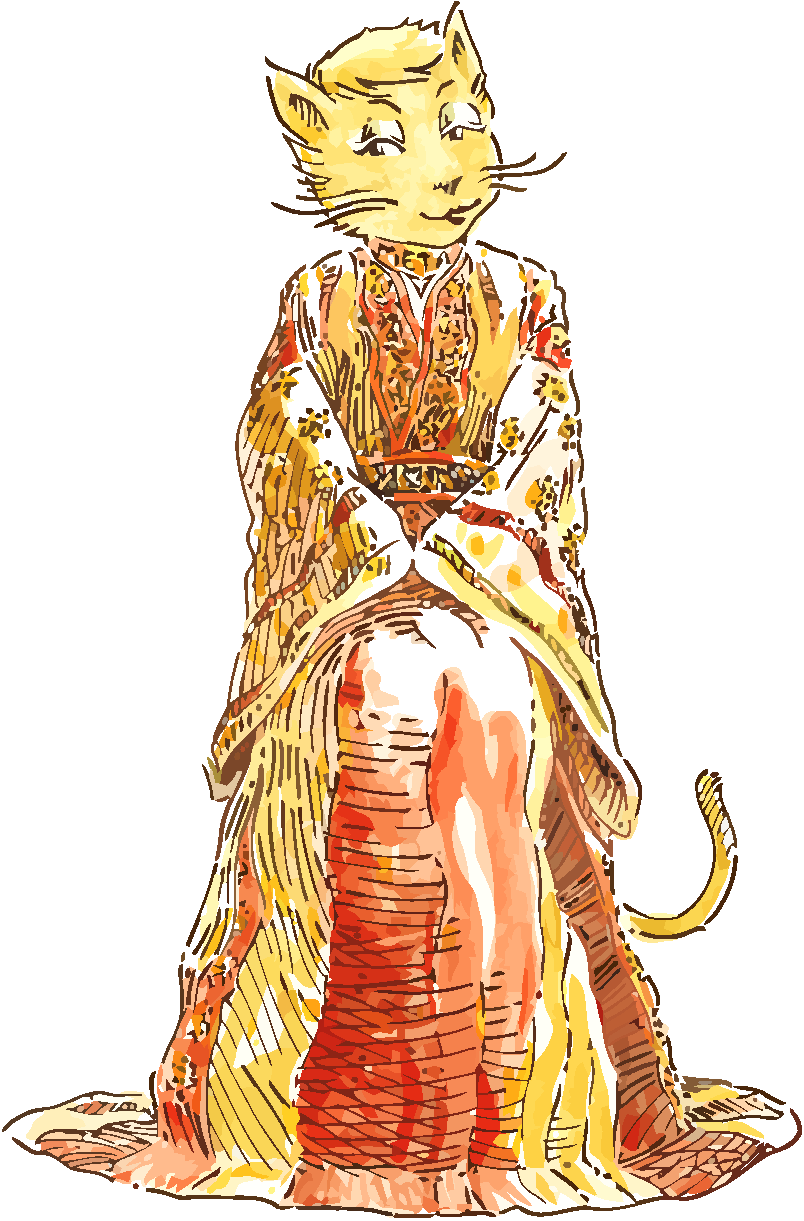
\includegraphics[height=3cm]{meta.pdf}}


%%
\begin{document}

\maketitle


%
\begin{frame}{매크로 관련 명령어}
  \vspace{4mm}
  \hbox to\hsize{\hss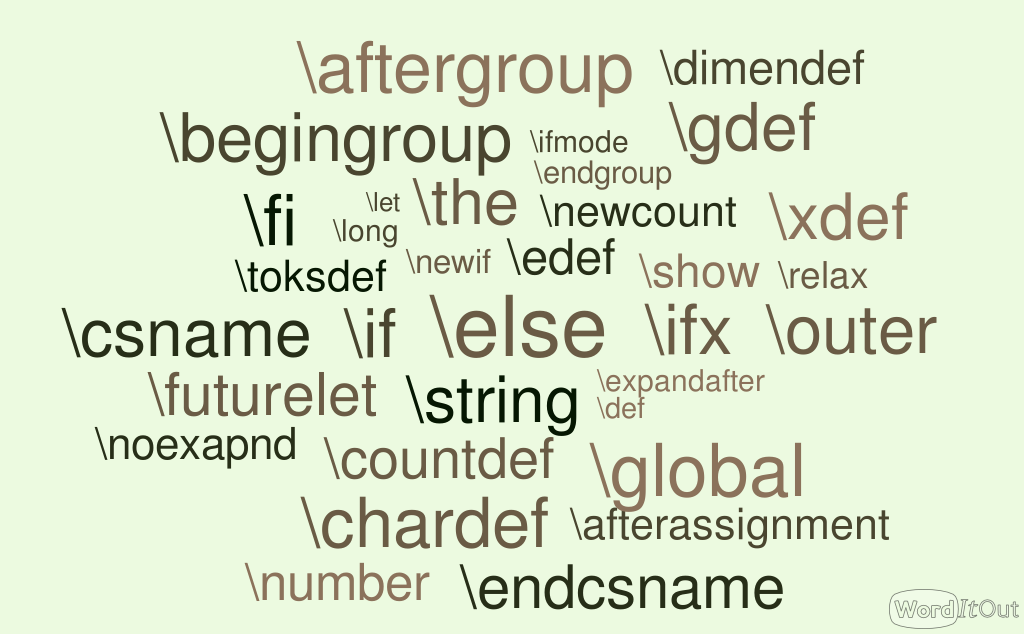
\includegraphics[height=7.5cm]{cs.png}\hss}
\end{frame}


%
\begin{frame}[fragile]{매크로 사용자 단계}
  The \TeX\ Hierarchy, TUGboat, Volume 15 (1994), No.1, 7---9.
  \begin{description}
  \item [Novice] has heard of macros, but has never seen one.
  \item [User] writes macros that are used once, and that are
    longer than the code they replace.
  \item [Programmer], having been bitten by unwanted spaces,
    writes macros that don't contain spaces, and every line ends with
    a `{\small\verb+%+}'.
  \item [Hacker] has written self-modifying macros, writes
    {\small\verb+\endlinechar=-1+} or {\small\verb+\catcode'\^^M=9+}
    to prevent having to put {\small\verb+%+}'s at the end of lines in macros.
  \item [Guru] has written macros containing {\small\verb+####+}, more than 3
    {\small\verb+\expandafter+}'s in a row, and the sequence
    {\small\verb+\expandafter\endcsname+}.
  \end{description}
\end{frame}


%
\begin{frame}[fragile]{매크로 정의}
  \medskip
  \hbox to\hsize{\hss
    \verb+\def+<control sequence>\alert{<parameter text>}%
    \verb+{+\alert{<replacement text>}\verb+}+\hss}
  \smallskip
  \begin{itemize}
  \item 문서에서 여러번 반복적으로 사용되는 문구나 명령어의 나열을 하나의
    명령어(control sequence)로 만든 것
  \item \verb+\def+, \verb+\gdef+, \verb+\edef+, \verb+\xdef+
  \item 텍의 전개 과정에서 매크로는 치환문으로 교체된다.
  \item 정의 시점에는 전개하지 않는다.
  \item 파라미터 텍스트와 치환 텍스트에는 정의되지 않은 매크로 사용이 가능하다.
    
    \verb+\def\control#1\sequence{...}+
  \item 매크로를 전개하기 위해서 인자를 읽어 들일때는 전개하지 않는다.
  \end{itemize}
\end{frame}


%
\begin{frame}{텍의 처리 과정}  
  \begin{itemize}
  \item \alert{\bf 입력(Input)} 파일을 줄(line) 단위로 읽어서
    \alert{토큰 리스트}를 만든다.
  \item \alert{\bf 전개(Expansion)} 위의 토큰 리스트를 입력으로 받어서 전개할 수 있는
    모든 토큰을 전개해서 더이상 전개 할 수 없는 토큰들로 구성된 새로운 토큰 리스트를 만든다.
  \item \alert{\bf 실행(Execution)}
  \item \alert{\bf 출력(Visual)}
  \end{itemize}
\end{frame}


%
\begin{frame}[fragile]{토큰 리스트}
  \alert{입력 과정}
  
  \verb*+{\hskip 36 pt}+\\
  \bigskip
  \verb|{|$_1$\quad\fbox{hskip}\quad\verb|3|$_{12}$
  \quad\verb|6|$_{12}$\quad
  \verb*| |$_{10}$\quad\verb|p|$_{11}$\quad\verb|t|$_{11}$\quad\verb|}|$_{2}$
\end{frame}


%
\begin{frame}[fragile]{토큰 리스트}
\begin{verbatim*}
\def\mytoken{\iftrue this \else that \fi}
\mytoken
\end{verbatim*}
    \bigskip
    \alert{입력 과정}
    
    \fbox{mytoken}
    
    \bigskip
    \alert{전개 과정}
    
    \fbox{iftrue}\quad
    \verb|t|$_{12}$\quad
    \verb|h|$_{12}$\quad
    \verb|i|$_{12}$\quad
    \verb|s|$_{12}$\quad
    \verb*| |$_{10}$\quad
    \fbox{else}\quad
    \verb|t|$_{12}$\quad
    \verb|h|$_{12}$\quad
    \verb|a|$_{12}$\quad
    \verb|t|$_{12}$\quad
    \verb*| |$_{10}$\quad
    \fbox{fi}

    \bigskip
    \verb|t|$_{12}$\quad
    \verb|h|$_{12}$\quad
    \verb|i|$_{12}$\quad
    \verb|s|$_{12}$\quad
    \verb*| |$_{10}$\quad
\end{frame}


%
\begin{frame}[fragile]{토큰 리스트}
\begin{verbatim*}
\def\tokentwo{\iftrue this \else that \fi}
\def\tokenone#1{...}
\expandafter\tokenone\tokentwo
\end{verbatim*}
    \bigskip

    \alert{입력 과정}
    
    \fbox{expandafter}\quad
    \fbox{tokenone}\quad
    \fbox{tokentwo}
    
    \bigskip
    \alert{전개 과정}

    \fbox{tokenone}\quad
    \verb|t|$_{12}$\quad
    \verb|h|$_{12}$\quad
    \verb|i|$_{12}$\quad
    \verb|s|$_{12}$\quad
    \verb*| |$_{10}$\quad (X)

    \bigskip
    \fbox{tokenone}\quad
    \fbox{iftrue}\quad
    \verb|t|$_{12}$\quad
    \verb|h|$_{12}$\quad
    \verb|i|$_{12}$\quad
    \verb|s|$_{12}$\quad
    \verb*| |$_{10}$\quad
    \fbox{else}\quad
    \verb|t|$_{12}$\quad
    \verb|h|$_{12}$\quad
    \verb|a|$_{12}$\quad
    \verb|t|$_{12}$\quad
    \verb*| |$_{10}$\quad
    \fbox{fi}
\end{frame}


%
\begin{frame}[fragile]{그룹 만들기}
  \textbf{\alert{그룹}}
  \begin{itemize}
  \item \verb+{+, \verb+}+
  \item \verb+\bgroup+, \verb+\egroup+
    ({\small \verb+\let\bgroup={ \let\egroup=}+})
  \item \verb+\begingroup+, \verb+\endgroup+
    \begin{alertblock}{사용례}
      \begin{itemize}
      \item \verb+\bgroup \bf Hello}+
      \item \verb+{\bf Hello \egroup+
      \end{itemize}
    \end{alertblock}
  \item \verb+\begingroup+, \verb+\endgroup+ (원시명령어, primitive)
  \end{itemize}

  {\small
\begin{verbatim}
    \def\hello{Hello}
    { \baselineskip=14pt \def\hello{Hola} \hello }
    \hello
\end{verbatim}}

  Hola Hello
\end{frame}


%
\begin{frame}[standout]
  예제
\end{frame}


%
\begin{frame}[fragile]{\texttt{\string\bold} 매크로}
\begin{verbatim}
    {\bf Hello world}
    
    \bold{Hello world}
\end{verbatim}
  \begin{alertblock}{Programmer}
    \verb+\def\bold#1{{\bf #1}}+
  \end{alertblock}
\end{frame}


%
\begin{frame}[fragile]{\texttt{\string\bold} 매크로}
\begin{verbatim}
    \bold{
      Hello

      world
    }

    Runaway argument?
    { Hello
    ! Paragraph ended before \bold was complete.
\end{verbatim}
  \begin{alertblock}{Programmer first class}
    \verb+\long\def\bold#1{{\bf #1}}+
  \end{alertblock}
\end{frame}


%
\begin{frame}[fragile]{\texttt{\string\bold} 매크로}
  \begin{alertblock}{Hacker}
    \verb+\def\beginbold{\bgroup\bf}+
    
    \verb+\def\endbold{\egroup}+
  \end{alertblock}

\begin{verbatim}
    \beginbold
    Hello

    world
    \endbold
\end{verbatim}
\end{frame}


%
\begin{frame}[fragile]{\texttt{\string\bold} 매크로}
  \begin{alertblock}{Wizard}
    \verb+\def\bold{\bgroup\bf\let\next=}+
  \end{alertblock}

\begin{verbatim}
bold{text}
\bgroup\bf\let\next={text}
\end{verbatim}

  \hbox to\hsize{\hss
    \verb+\let+<control sequence><equals>%
    <one optional space><token>\hss}
  <equals>$\rightarrow$<optional spaces> | <optional spaces>=

\bigskip

  \fbox{bgroup}\quad\fbox{bf}\quad
  \verb|t|$_{11}$\quad\verb|e|$_{11}$\quad
  \verb|x|$_{11}$\quad\verb|t|$_{11}$\quad
  \verb|}|$_{2}$

  \verb|{|$_1$\quad\fbox{bf}\quad
  \verb|t|$_{11}$\quad\verb|e|$_{11}$\quad
  \verb|x|$_{11}$\quad\verb|t|$_{11}$\quad
  \verb|}|$_{2}$
\end{frame}


%
\begin{frame}[fragile]{스크립트 매크로}
\begin{verbatim}
  \beginscript
  Now, at last, you can easily typeset
  conversations you eavesdrop on in
  restaurants and on planes.
  
  Really? That's just what I've been waiting
  for! How do I do it?
  
  Exactly the way this script was done.
  
  Is it easy?
  
  Extremely.
  \endscript
\end{verbatim}
\end{frame}


%
\newcount\spk
\def\beginscript{\bgroup \parindent=0pt \rm \spk=1 \rightskip.4in
  \def\par{\ifnum\spk=1 \endgraf \sl \spk=2 \leftskip.4in \rightskip0in
    \else \endgraf \rm \spk=1 \leftskip0in \rightskip.4in \fi}}
\def\endscript {\egroup}

\begin{frame}[fragile]{스크립트 매크로}
  \hsize 3in
  \beginscript
  Now, at last, you can easily typeset
  conversations you eavesdrop on in
  restaurants and on planes.
  
  Really? That's just what I've been waiting
  for! How do I do it?
  
  Exactly the way this script was done.
  
  Is it easy?
  
  Extremely.
  \endscript
\end{frame}


%
\begin{frame}[fragile]{스크립트 매크로}
\begin{verbatim}
  \let\endgraf=\par
  \newcount\spk
  \def\beginscript{\bgroup \parindent=0pt \rm
    \spk=1 \rightskip.4in
    \def\par{\ifnum\spk=1 \endgraf \sl \spk=2
               \leftskip.4in \rightskip0in
             \else \endgraf \rm \spk=1
               \leftskip0in \rightskip.4in \fi}}
  \def\endscript{\egroup}
\end{verbatim}
\end{frame}


%
\begin{frame}[fragile]{FIFO 매크로}
\begin{verbatim}
    \def\fifo#1{\ifx\ofif#1\ofif\fi
      \process#1\fifo}
    \def\ofif#1\fifo{\fi}

    \fifo abc\ofif
    => \process a \process b \process c
\end{verbatim}
\end{frame}


%
\begin{frame}[fragile]{FIFO 매크로}
\begin{verbatim}
    \def\fifo#1{\ifx\ofif#1\ofif\fi
      \process#1\fifo}
    \def\ofif#1\fifo{\fi}

    \newcount\length
    \def\process#1{\advance\length 1}

    \fifo aapnoon\ofif \number\length % => 7
\end{verbatim}
\end{frame}


%
\begin{frame}{참고 문서}
  \begin{itemize}
  \item \href{http://ftp.ktug.org/tex-archive/systems/knuth/dist/tex/}
    {The \TeX book}
  \item \href{http://ftp.ktug.org/tex-archive/info/impatient/book.pdf}
    {\TeX\ for the Impatient}
  \item \href{http://ftp.ktug.org/tex-archive/info/texbytopic/TeXbyTopic.pdf}
    {\TeX\ By Topic}
  \item \href{http://pgfplots.sourceforge.net/TeX-programming-notes.pdf}
    {Notes On Programming in TeX}
  \item \href{https://www.tug.org/TUGboat/tb14-1/tb38laan.pdf}
    {FIFO and LIFO sing the BLUes}
  \item \href{https://www.tug.org/TUGboat/tb08-3/tb19knut.pdf}
    {Macros for Jill}
  \item \href{https://www.tug.org/TUGboat/tb15-1/tb42arseneau.pdf}
    {The TeX\ Hierarchy}
  \end{itemize}
\end{frame}


%
\begin{frame}[standout]
  ¿Tienes alguna pregunta?
\end{frame}

\end{document}
